\chapter{Introduction and Contributions}
\label{chapt:intro}

\blfootnote{Portions of this chapter previously appeared as: \nobibentry{me:mascots:2012}}

An introduction to the thesis.
Despite the footnote, here is my first citation~\cite{jefferson-tw}.

I think it is tacky to have a section without an intro text.

\section{Circuit Design}

I have a pretty image, see Figure~\ref{fig:design-process}.

\begin{figure*}[ht]
\centering
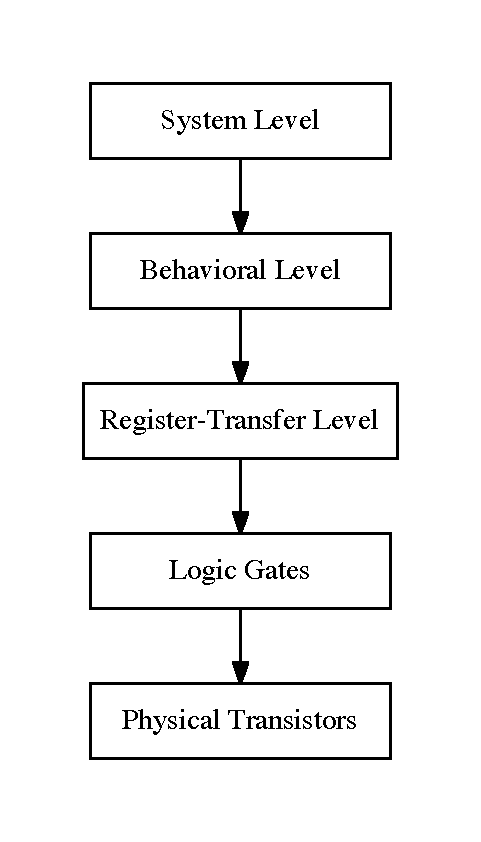
\includegraphics[width=0.4\textwidth]{figs/cdp.pdf}
\caption [Circuit Design Process Levels of Abstraction] {
	Levels of abstraction within the circuit design process.
	Automatic tools perform synthesis on a given design to generate the design at the next (lower) level.
	This design is then validated through one or more tests.
}
\label{fig:design-process}
\end{figure*}




\section{Contributions}

You thesis committee is very smart.
Prove that you are smart by clearly stating what your contributions are.

\subsection{Contribution 1: Publication 1}

I did a thing and published the work.

\subsection{Contribution 2: Other thing}

Some other thing I did.

\subsection{Contribution 3: Final Thing}

Also this.

\section{Thesis Organization}

This document begins by presenting the necessary background (include domain specific terminology and related works) for understanding my contributions (Chapter~\ref{chapt:bg}).
I then present a working proof-of-concept experiment (Chapter~\ref{chapt:pub1}).
The challenges faced in this proof-of-concept experiment lead to my research on three distinct problems:
\begin{itemize}
  \item Thing A (Chapter~\ref{chapt:a});
  \item Thing B (Chapter~\ref{chapt:b});
  \item Thing C (Chapter~\ref{chapt:c});
\end{itemize}
Finally, I present my research contributions and discuss the conclusions drawn from these experiments (Chapter~\ref{chapt:conc}).
